% Op icon: helix — a coil/spring viewed from the side, dashed centre axis.
\documentclass[tikz,border=2mm]{standalone}
\usetikzlibrary{arrows.meta,calc,shapes.geometric}
\begin{document}
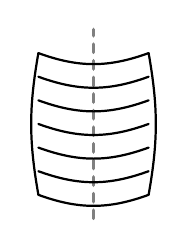
\begin{tikzpicture}[line width=1.3pt, line cap=round, line join=round, >=Stealth, x=1mm,y=1mm]
  \draw[dashed, gray] (0,-12) -- (0,12);
  \foreach \y in {-9,-6,-3,0,3,6,9} { \draw[thick] (-7,\y) to[out=-20,in=200] (7,\y); }
  \draw[thick] (-7,-9) to[out=100,in=-100] (-7,9);
  \draw[thick] (7,-9) to[out=80,in=-80] (7,9);
\end{tikzpicture}
\end{document}
